\section{Misión SAOCOM y aplicaciones}
\subsection{Misión SAOCOM}

\begin{frame}{\secname : \subsecname}
  \begin{figure}
    \centering
    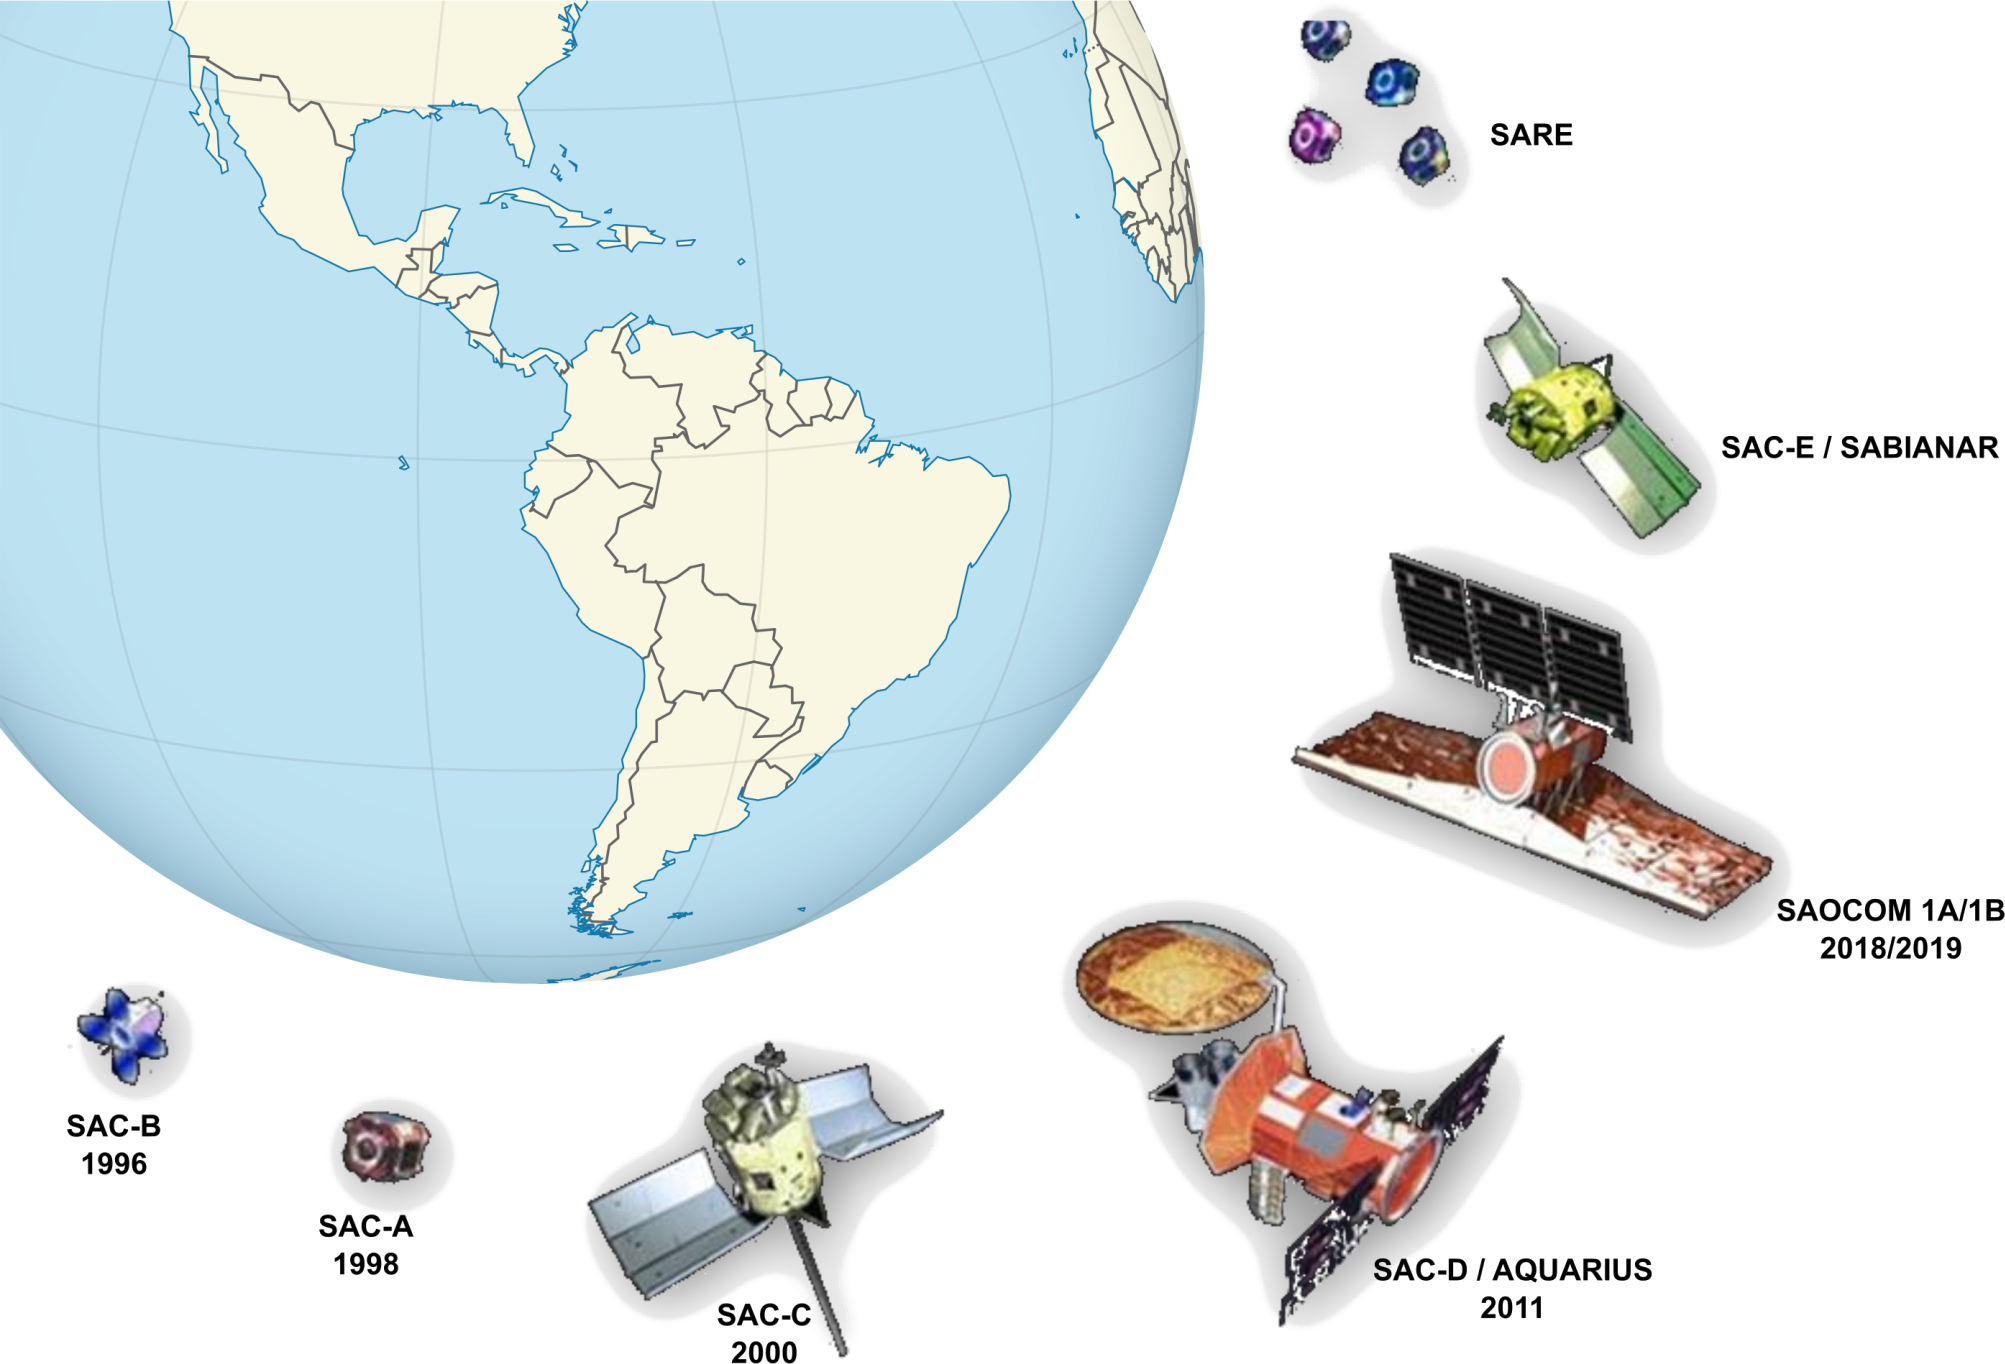
\includegraphics[width=0.65\textwidth]{fig:plan}
    \caption{Satélites del plan espacial nacional.}
    \label{}
  \end{figure}
\end{frame}
%--- Next Frame ---%

\begin{frame}{\secname : \subsecname}
  \begin{figure}
    \centering
    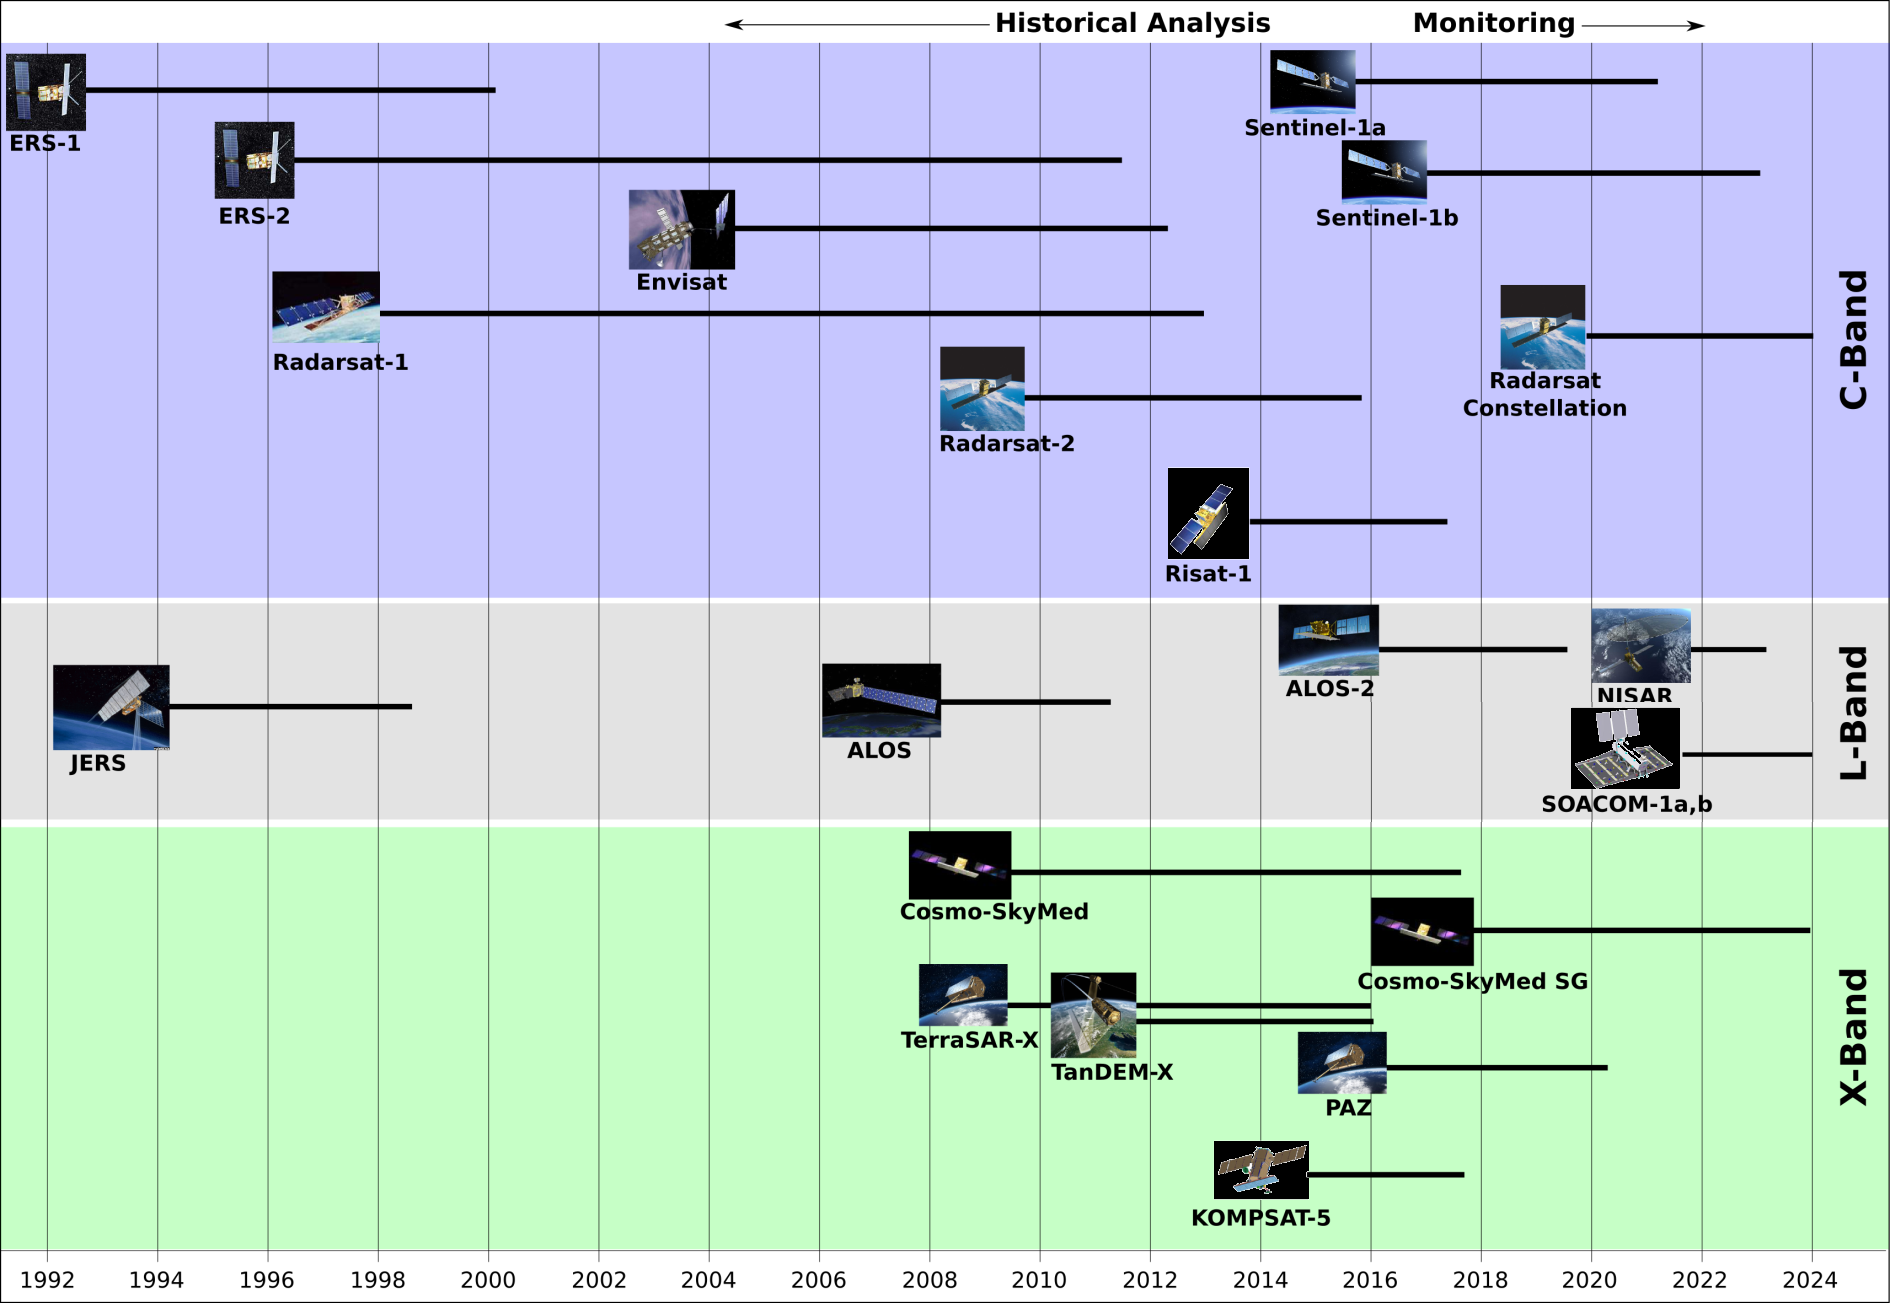
\includegraphics[width=0.7\textwidth]{fig:misiones}
    \caption{Misiones satelitales históricas y actuales.}
    \label{}
  \end{figure}
\end{frame}
%--- Next Frame ---%



\begin{frame}{\secname : \subsecname}
  \begin{columns}
    \begin{column}{0.6\textwidth}
     \begin{block}{Mision SAOCOM}
\begin{itemize}
  \item Dos satélites idénticos
  \item L-Band SAR (1275 Mhz)
  \item Cobertura Global
  \item Mirada a derecha
  \item Mirada a izquierda
  \begin{itemize}
    \item Hasta 5 minutos
  \end{itemize}
  \item Antena activa de 10m x 3.5m con 140 MTR
\end{itemize}
     \end{block}
    \end{column}
    \begin{column}{0.4\textwidth}  %%<--- here
      \begin{figure}
        \centering
        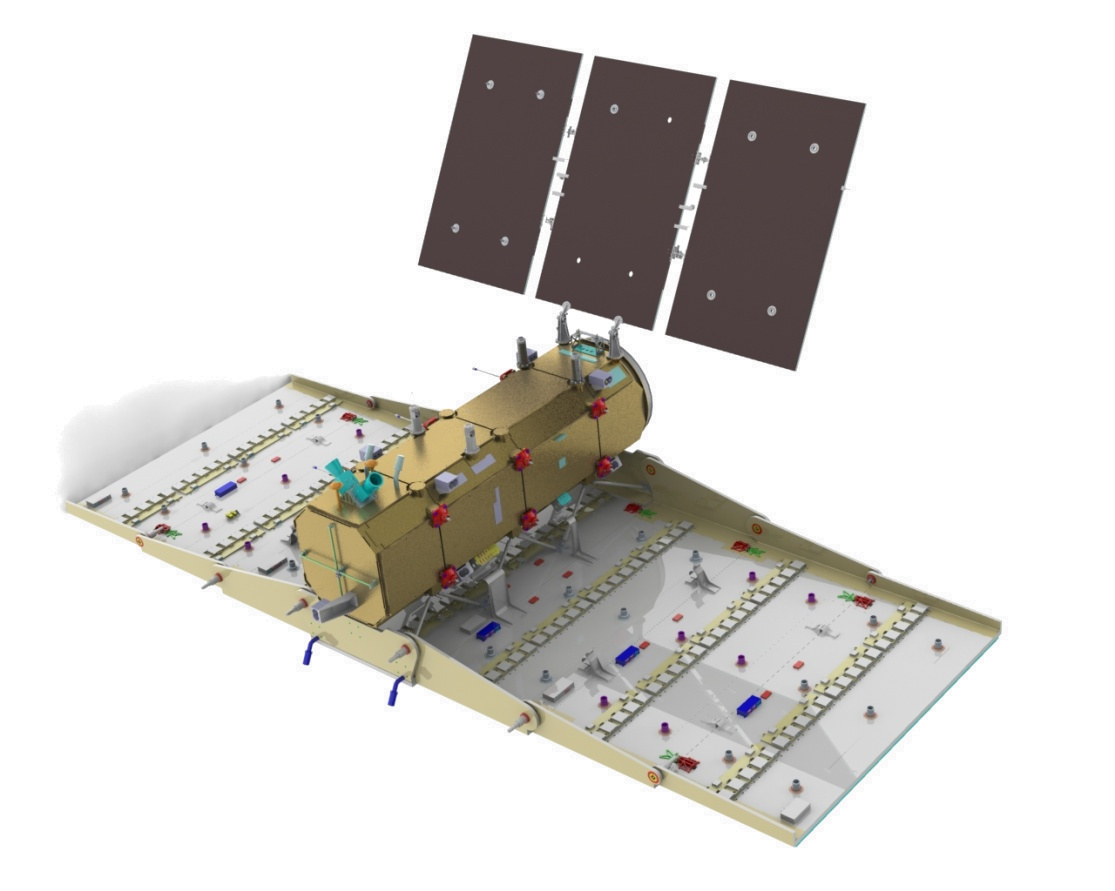
\includegraphics[width=1.1\textwidth]{fig:saocom.jpg}
        \caption*{}
        \label{}
      \end{figure}
    \end{column}
    \end{columns}

\end{frame}
%--- Next Frame ---%

\begin{frame}{\secname : \subsecname}
  \begin{columns}
    \begin{column}{0.6\textwidth}
     \begin{block}{Mision SAOCOM}
\begin{itemize}
  \item Órbita polar, heliosincrónica (inclinación 97.89) a 620 km de altura.
  \item Cada satélite esta desfasado 180 grados.
  \item Hora local de pasada por el Ecuador en forma ascendente: 6:12 am.
  \item Duración de la orbita 97.2 minutos.
  \item Tiempo de revisita: 16 días (1 satélite)/8 días (constelación)
  \item Órbitas por ciclo: 237.
  \item 23 ciclos por año
\end{itemize}
     \end{block}
    \end{column}
    \begin{column}{0.4\textwidth}  %%<--- here
      \begin{figure}
        \centering
        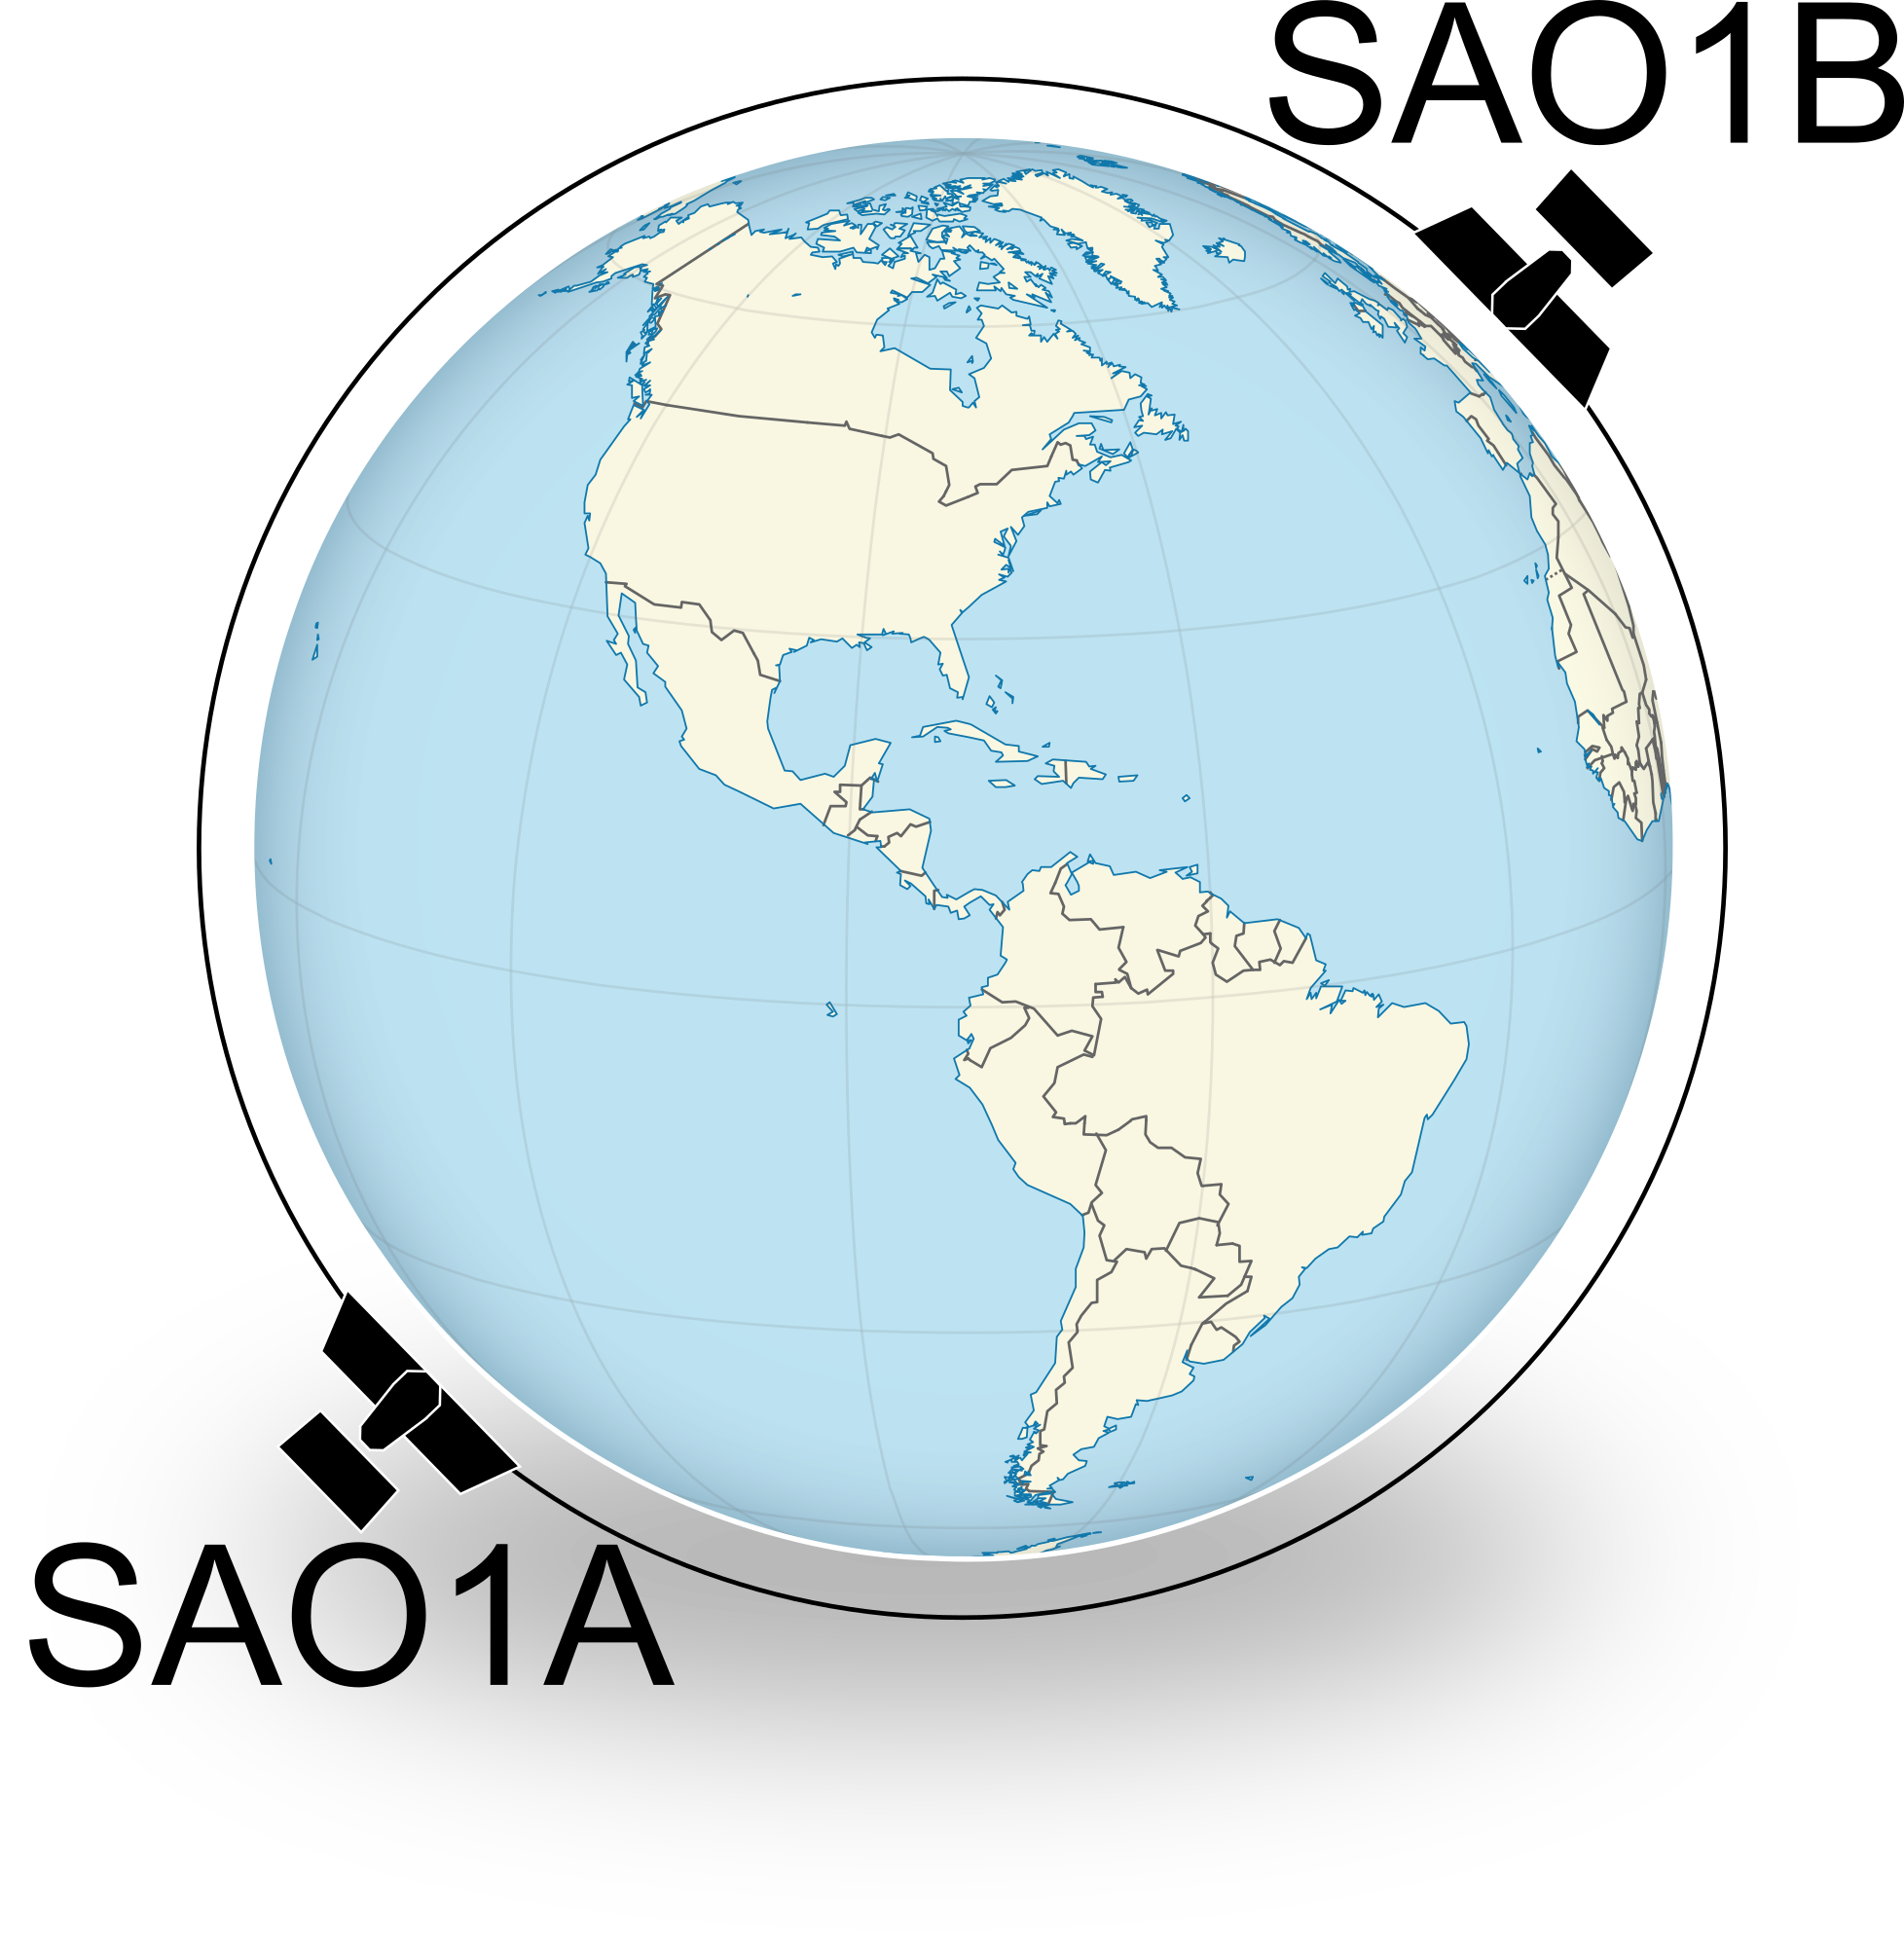
\includegraphics[width=1.1\textwidth]{fig:costelacion.png}
        \caption*{}
        \label{}
      \end{figure}
    \end{column}
    \end{columns}

\end{frame}
%--- Next Frame ---%

\subsection{Aplicaciones SAR}

\begin{frame}{\secname : \subsecname}
  \begin{figure}
    \centering
    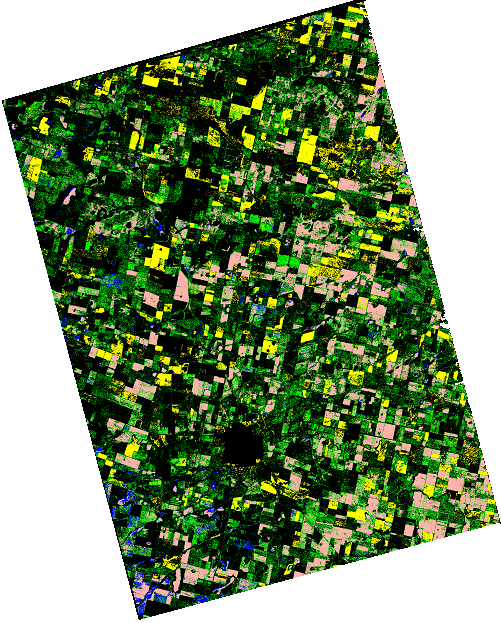
\includegraphics[width=0.35\textwidth]{fig:class.png}
    \caption{Clasificación de cultivos. Rosa: Suelo desnudo, Amarillo: Maiz, Verde: Soja, Agua: Azul, Negro, sin dato. Cosmo SkyMed.}
    \label{}
  \end{figure}
\end{frame}
%--- Next Frame ---%

\begin{frame}{\secname : \subsecname}
  \begin{figure}
    \centering
    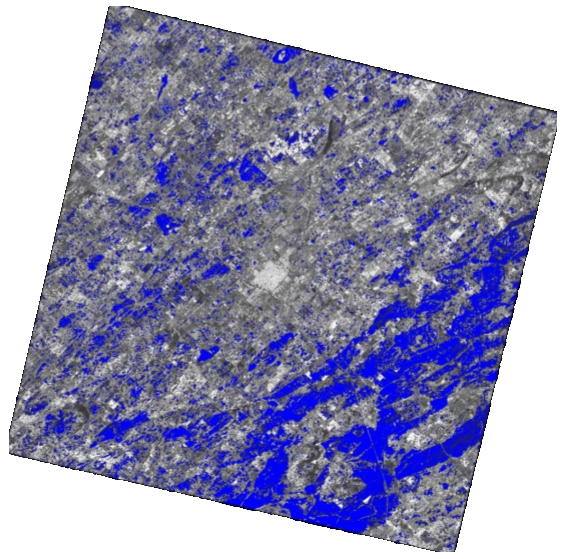
\includegraphics[width=0.48\textwidth]{fig:agua.png}
    \caption{Detección de cuerpos de agua. 19 de agosto de 2017. Cosmo SkyMed.}
    \label{}
  \end{figure}
\end{frame}
%--- Next Frame ---%

\begin{frame}{\secname : \subsecname}
  \begin{figure}
    \centering
    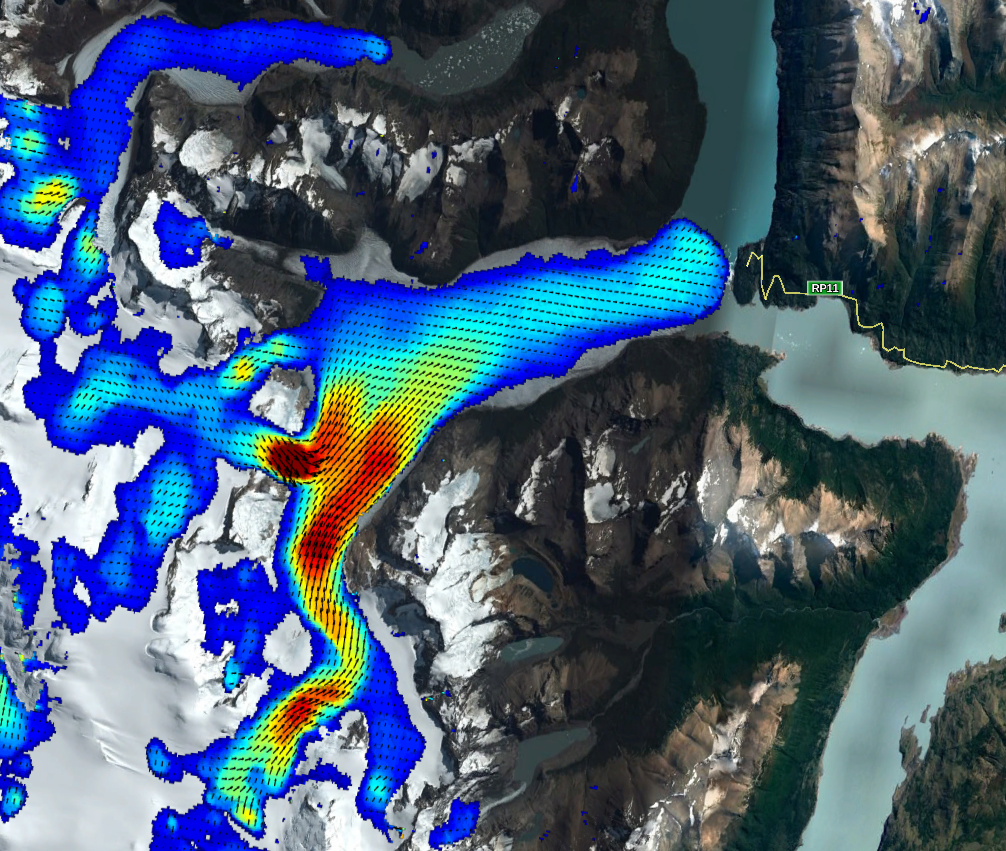
\includegraphics[width=0.5\textwidth]{fig:glaciar.png}
    \caption{Velocidad de desplazamiento de glaciares. Glaciar Perito Moreno. COSMO-SkyMed.}
    \label{}
  \end{figure}
\end{frame}
%--- Next Frame ---%

\begin{frame}{\secname : \subsecname}
  \begin{figure}
    \centering
    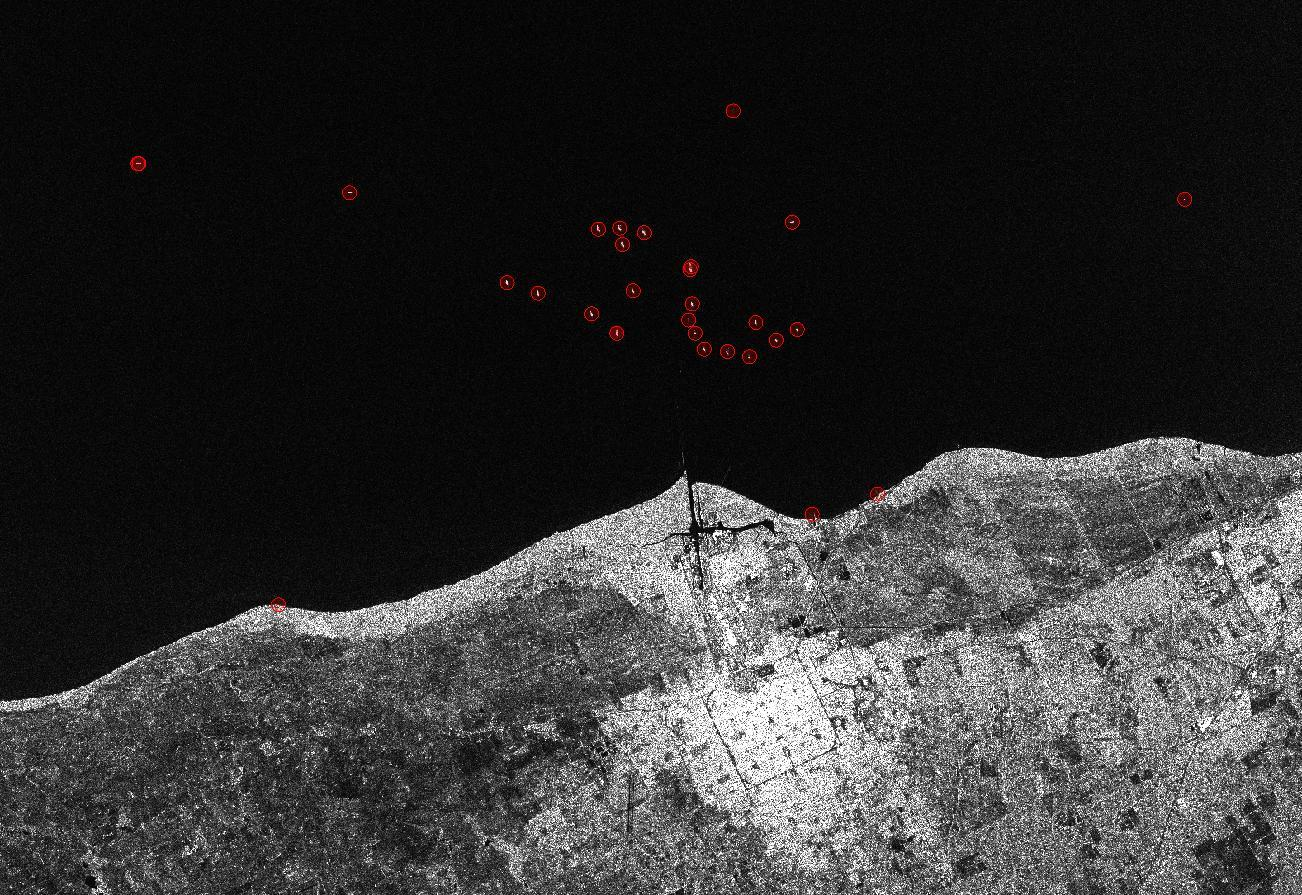
\includegraphics[width=0.6\textwidth]{fig:barcos.jpg}
    \caption{Detección de barcos frente a la ciudad de La Plata. 6 de diciembre de 2017. Sentinel 1.}
    \label{}
  \end{figure}
\end{frame}
%--- Next Frame ---%

\begin{frame}{\secname : \subsecname}
  \begin{figure}
    \centering
    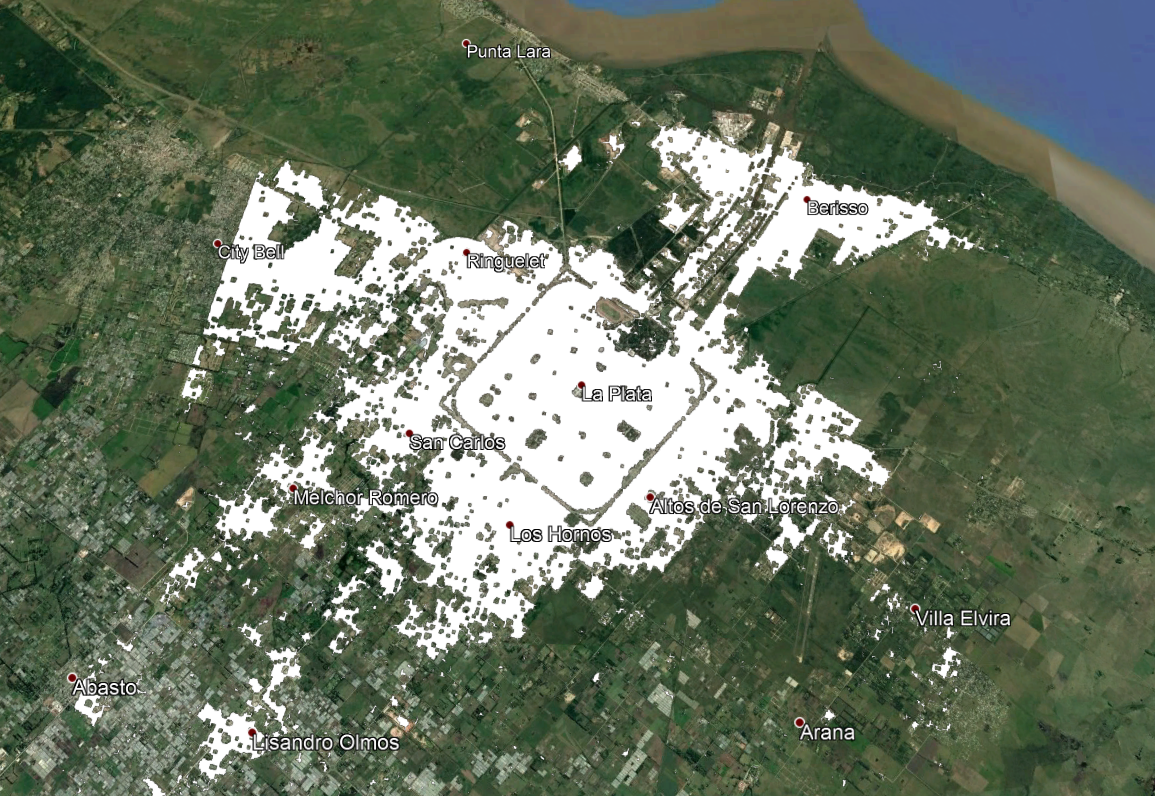
\includegraphics[width=0.6\textwidth]{fig:expansion.png}
    \caption{Detección de áreas urbanas. Ciudad de La Plata y alrededores.}
    \label{}
  \end{figure}
\end{frame}
%--- Next Frame ---%

\begin{frame}{\secname : \subsecname}
  \begin{figure}
    \centering
    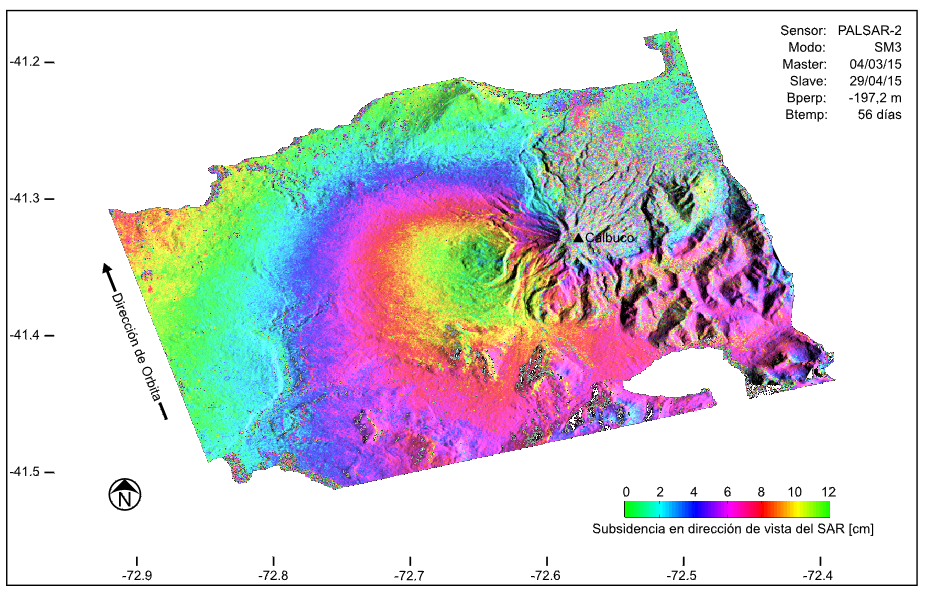
\includegraphics[width=0.65\textwidth]{fig:volcan.png}
    \caption{Deformación de la superficie por erupción del Volcán Calbuco, 22 de abril de 2015. Imagen ALOS PALSAR 2.}
    \label{}
  \end{figure}
\end{frame}
%--- Next Frame ---%

\begin{frame}{\secname : \subsecname}
  \begin{figure}
    \centering
    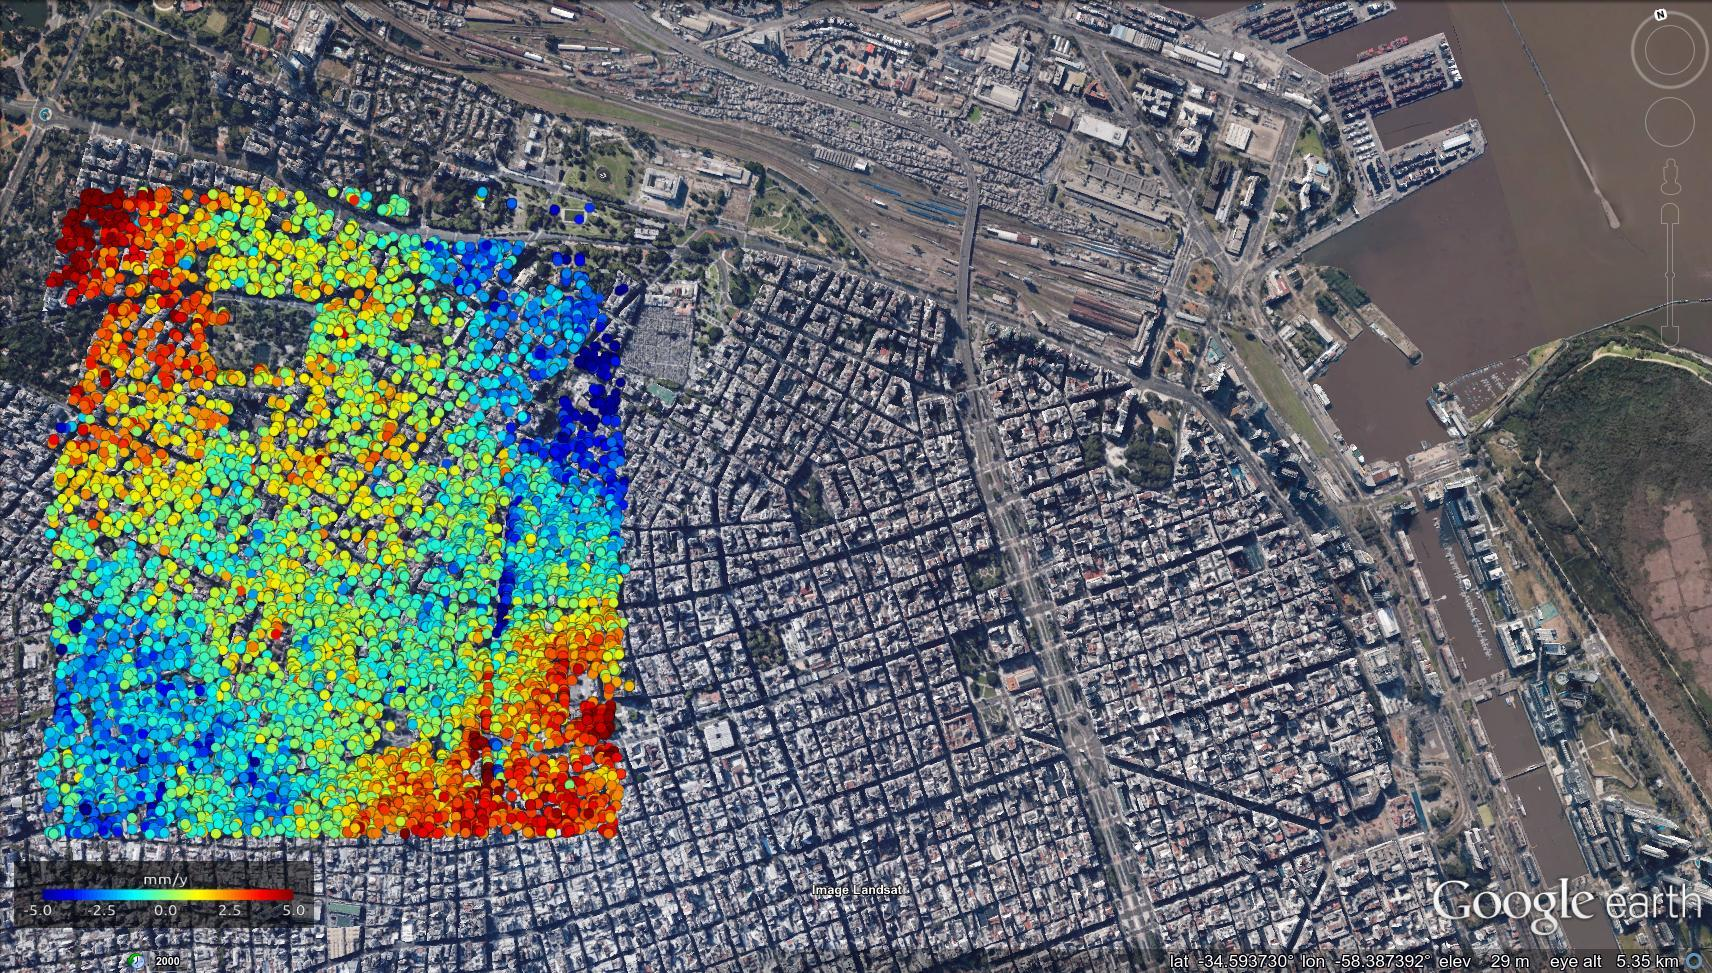
\includegraphics[width=0.75\textwidth]{fig:subduccion.jpg}
    \caption{Detección de subsidencia por métodos interferométricos.}
    \label{}
  \end{figure}
\end{frame}
%--- Next Frame ---%

\begin{frame}{\secname : \subsecname}
  \begin{figure}
    \centering
    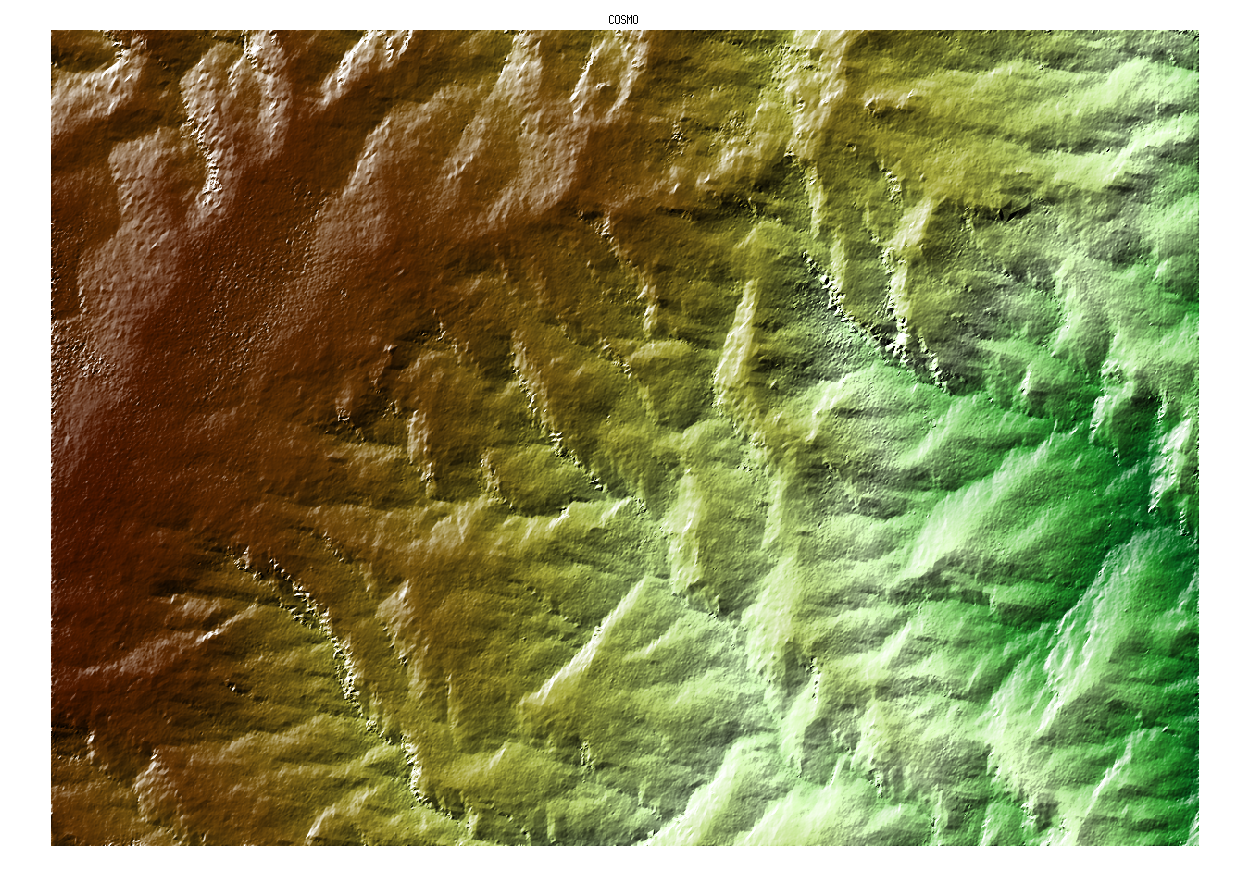
\includegraphics[width=0.65\textwidth]{fig:dem.png}
    \caption{Modelo digital de elevación (DEM). Cosmo SkyMed.}
    \label{}
  \end{figure}
\end{frame}
%--- Next Frame ---%


\begin{frame}{\secname : \subsecname}
Muchas gracias.
\end{frame}
%--- Next Frame ---%
